%% Define document class, variables and frontmatter
\documentclass{beamer}
\usepackage{tikz}
\title{Project report}
\def\showoutlineatsection{true}
%%% Variables, functions and other settings
%% Define beamer theme
\usetheme{Goettingen}
%% Packages
%\usepackage[utf8]{inputenc}
%\usepackage[T1]{fontenc}
%% Define basic variables
\subtitle{}
\author{Neronet}
\institute[]{
  \emph{
    Toolbox for managing the training \\
    neural networks
  } \\[0.5cm]
  CSE-C2610 \\
  Software Project \\[0.2cm]
  Aalto University
}
\date{\today{}}
\subject{Software engineering}
%% Colors and visuals
% Specify link and URL colors
\hypersetup{colorlinks,linkcolor=,urlcolor=magenta}
% Replace navigation symbols with a logo
\logo{
\includegraphics[height=1cm]{gfx/logo_aalto.png}}
\setbeamertemplate{navigation symbols}{\insertlogo}
%% Functions
% Define short set and clear background commands
\newcommand{\bgset}[1]{\usebackgroundtemplate{
  \includegraphics[width=\paperwidth,height=\paperheight]{#1}}}
\newcommand{\bgclear}{\usebackgroundtemplate{}}
\ifdefined \showoutlineatsection
  % Have LaTeX render an outline frame just before each new section
  \AtBeginSection[]{
    \bgset{gfx/neural3__bgmod.jpg}
    \begin{frame}<beamer>{Outline}
      \tableofcontents[currentsection]
    \end{frame}
    \bgset{gfx/neural1__bgmod.jpg}}
\fi
%%% Main document content
\begin{document}
%% Title page
\bgset{gfx/neural2__bgmod.jpg}
\begin{frame}
  \titlepage
\end{frame}
%% Outline page
\bgset{gfx/neural3__bgmod.jpg}
\begin{frame}{Outline}
  \tableofcontents
\end{frame}
\def\Done{\textcolor{green}{Done}}
\def\Undone{\textcolor{red}{Undone}}
%% Structure
% ---- INTRO
% #) Pyry's statement as an interest booster: best group so far, professional results
% #) Team -- team photo, description
% #) Pyry -- photo of Pyry, role, background
% ---- PROJECT
% #) Pyry's problem; our challenge
% #) Vision
% #) Technical challenges, ASRs
% #) Solution -- architecture
% #) Outcome summary: what Neronet can do now?
% #) Demo
% ---- PROCESS
% #) Process overview; schedule; used tools
% #) Definition of done
% #) Testing and QA
% #) Overview of sprints: goals
% #) Stories done by sprint and sprint goals; challenges and found solutions
% #) Peer team feedback
% #) User feedback
% #) Quality attributes
% #) Retrospective summaries
% #) Overall project summary
% #) Overall project challenges: Pyry, topic, experience
% #) Summary of technical and sprint challenges and solutions
% #) Future as an OS project
% #) Thanks to our team, Eero, Pyry, Simo, Jelena, course staff
% Notes:
% - Lots of content: We have to train a lot in order to fit it all into 35 minutes.
% - Key things to mention must be printed on paper
%% Content pages


\begin{frame}{Forecitation}
  I have supervised several bachelors' theses and other student projects.

  \vspace*{1cm}
  You surprised me with your \alert{commitment} and \alert{effort}.

  \vspace*{1cm}
  Pyry Takala, PO
\end{frame}

\section{People} \bgset{gfx/neural2__bgmod.jpg}

\begin{frame}{Team}
  \begin{figure}
    \centering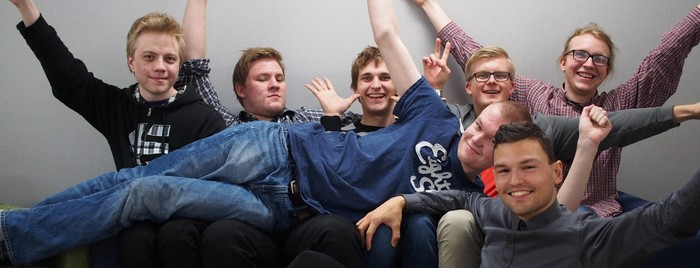
\includegraphics[width=1\columnwidth]{gfx/team.jpg}
  \end{figure}
  At the start of the course, we were all both
  \begin{itemize}
  \item \alert{terrified}, and 
  \item \alert{inspired}
  \end{itemize}
  by our project topic!
\end{frame}
\begin{frame}{Product owner}
  \begin{figure}
    \centering
\includegraphics[width=0.4\columnwidth]{gfx/pyry.jpg}
  \end{figure}
  \begin{itemize}
  \item Machine learning researcher at Aalto
  \item Past: Amazon, McKinsey \& Company, Goldman Sachs, August...
  \item A great PO!
  \end{itemize}
\end{frame}
\begin{frame}{Agile coach}
  \begin{figure}
    \centering
\includegraphics[width=0.4\columnwidth]{gfx/eero.jpg}
  \end{figure}
  \begin{itemize}
  \item Continuous Delivery researcher at Aalto
  \item Past: Prosys PMS Ltd, WiRCA-miehet, Aalto...
  \item A great coach!
  \end{itemize}
\end{frame}

\section{Project} \bgset{gfx/neural1__bgmod.jpg}

\begin{frame}{Pyry's problem}
  Challenges in training neural networks
  \begin{itemize}
  \item Takes forever!
  \item Might anything be wrong?
  \item If yes, what?
  \item Is it developing better than its precedants?
  \item Why does it take forever?
  \end{itemize}
\end{frame}
\begin{frame}{Vision}
  A tool that would
  \begin{itemize}
  \item facilitate experiment management
  \item provide information on ongoing experiments
  \item be able to autoterminate experiments
  \item archive all results
  \item possibly even facilitate analysis
  \end{itemize}
\end{frame}
\begin{frame}{Vision}
  Other requirements
  \begin{itemize}
  \item lightweight
  \item easily extensible
  \item open source
  \item good usability
  \item framework agnostic
  \end{itemize}
\end{frame}
\begin{frame}{Journey map}
  \begin{figure}
  \tikzset{
    jmi/.append style={align=center,font=\tiny,shape=circle,draw,fill=gray!30,
    minimum size=1.4cm}, jmc/.style={font=\normalsize},
    man/.style={fill=blue!30}, mum/.style={draw=red,thick},
    kid/.style={fill=green!30}, nm/.style={color=blue},
    nj/.style={color=green}, jm/.style={color=red}
  }
  \resizebox{0.8\columnwidth}{!}{
  \begin{tikzpicture}
    \node (00)            [jmi,jmc]          {Research \\ journey};
    \node (01) at (180:4) [jmi]              {Innovate \\ ideas};
    \node (02) at (150:4) [jmi]              {Review \\ literature};
    \node (03) at (120:4) [jmi]              {Write \\ code};
    \node (04) at ( 90:4) [jmi,man]          {Embed \\ analytics};
    \node (05) at ( 60:4) [jmi,man]          {Design \\ tests};
    \node (06) at ( 30:4) [jmi,man,mum]      {Launch \\ tests};
    \node (07) at (  0:4) [jmi,kid,mum]      {Check \\ progress};
    \node (08) at (330:4) [jmi,kid,mum]      {Abort \\ failures};
    \node (09) at (300:4) [jmi,kid,mum]      {Collect \\ results};
    \node (10) at (270:4) [jmi,man]          {Analyse \\ results};
    \node (12) at (225:4) [jmi]              {Publish/drop \\ results};
    \foreach \a/\b in {00/01,01/02,02/03,03/04,04/05,05/06,06/07,07/08,08/09,09/10,10/01,10/12,12/00}
      \draw [->] (\a) edge (\b);
    \node (nm) at ( 30:2) [nm]               {\texttt{neroman}};
    \node (nm) at (  0:2) [jm]               {\texttt{neromum}};
    \node (nj) at (330:2) [nj]               {\texttt{nerokid}};
  \end{tikzpicture}
  }
  \end{figure}
\end{frame}
\begin{frame}{Technical challenges \& ASRs} % Joona
  \begin{itemize}
  \item deeply technical and an advanced domain
  \item remote computing nodes and cluster management
  \item good usability? according to whom?
  \item framework agnostic?
  \end{itemize}
\end{frame}

\section{Results}

\begin{frame}{Result}
  A three component tool involving Python, SSH and sockets
  that ... \alert{meets the vision}!

  \begin{itemize}
  \item All core functionality \Done{}.
  \item Most features accessible both via CLI and GUI.
  \item PO satisfied.
  \item We are proud!
  \end{itemize}
\end{frame}
\begin{frame}{Solution}
  \begin{figure}
  \tikzset{
    ndom/.style={align=left}
    ncmp/.style={align=center,font=\small,shape=circle,draw,minimum size=3cm},
    ncmp/.style={align=center,font=\small,shape=circle,draw,minimum size=3cm},
    nmum/.style={align=center,font=\small,shape=circle,draw,minimum size=2cm},
    njob/.style={align=center,font=\tiny,shape=circle,draw,fill=green!30},
  }
  \resizebox{0.8\columnwidth}{!}{
    \begin{tikzpicture}
      \draw[dashed] ( 0, 6  ) rectangle (11,11);
      \draw[dashed] ( 0, 0  ) rectangle (11, 5);
      \node (ln) at ( 2,10  ) [ndom]                 {Local network};
      \node (ln) at ( 2, 4  ) [ndom]                 {Cluster network};
      \node (nm) at ( 6, 9  ) [ncmp,fill=blue!30]    {\texttt{neroman}};
      \node (mm) at ( 6, 5.5) [nmum,fill=red!30]     {\texttt{neromum}};
      \node (j1) at ( 3, 2  ) [njob]                 {\texttt{nerokid}};
      \node (j2) at ( 5, 1  ) [njob]                 {\texttt{nerokid}};
      \node (j4) at ( 7, 1  ) [njob]                 {\texttt{nerokid}};
      \node (j3) at ( 9, 2  ) [njob]                 {\texttt{nerokid}};
      \foreach \a/\b in {nm/mm,mm/j1,mm/j2,mm/j3,mm/j4}
        \draw [<->] (\a) edge (\b);
    \end{tikzpicture}
  }
  \end{figure}
\end{frame}

\section{Demo}

\begin{frame}{Demo}
  Live demonstration of the final product including:
  %We have created video demo and would like to show it now.

  \begin{enumerate}
  \item Cluster \& experiment configuration
  \item Experiment submission
  \item Fetching updates/results
  \item Viewing plots
  \end{enumerate}

  Focus on the GUI this time.
\end{frame}
\begin{frame}{Recap}
  In essence the product is a Python-based tool that enables computational
  researchers to conduct their research more effectively.
  \begin{itemize}
  \item It utilizes SSH and TCP sockets to distribute computational
    experiments into remote computer nodes.
  \item It is framework agnostic in that it permits the use of a very wide
    variety of tools to actually conduct the computing needed (Theano, Torch,
    Scipy, Matlab, R, C++, whatever).
  \end{itemize}
\end{frame}
\begin{frame}{User feedback}
We utilized lots of end user testing and received great feedback from a
Triton admin:

\begin{itemize}
  \item Thought that our design and architecture was well devised.
  \item Offered performance improvement ideas.
  \item In general he liked our usability as did our PO.
\end{itemize}
\end{frame}

\section{Quality} \bgset{gfx/neural1__bgmod.jpg}

\begin{frame}{Quality}
  Quality assurance was based on

  \begin{itemize}
  \item the DoD, and
  \item our QA practices
  \end{itemize}

  We updated our DoD and practices several times.
\end{frame}
\begin{frame}{Definition of done}
  We defined \Done{} at the BI, sprint and project level.
    
  \begin{itemize}
  \item BI level: unit tests, code confromity, commenting, documentation, peer review
  \item Sprint level: BIs \Done{}, unit and system tests ok, sprint goal achieved.
  \item Project level: all sprints \Done{}.
  \end{itemize}
\end{frame}
\begin{frame}{QA practices}
  Used QA practices and tools:
  \begin{itemize}
  \item Unit test framework
  \item Commenting \& documentation
  \item System testing
  \item Peer review
  \end{itemize}
\end{frame}
\begin{frame}{Quality attributes}
  Added emphasis on these attributes:

  \begin{itemize}
  \item Usability
  \item Reliability
  \item Extendability
  \item Performance
  \end{itemize}
\end{frame}

\section{Process}

\begin{frame}{Process overview}
  \begin{itemize}
  \item Teamwork sessions almost every Wed \& Fri at Maari
  \item Scrum as required
  \item Tried to employ professional SD practices
  \item Tools: Github, Agilefant, Flowdock, WhatsApp, Google Calendar,
    ShareLaTeX, Skype, Floobits
  \end{itemize}
\end{frame}
\begin{frame}{Schedule}
  \begin{table} \small
  \begin{tabular}{lll}
    Time          & Event                     & Participants     \\ \hline
    30.10. 16-18  & Project kickoff           & team, PO         \\
    13.11. 15-17  & S0 demo                   & team, Coach      \\
    16.11. 11-13  & S1 planning               & team, PO         \\
    04.12. 16-17  & S1 \& progress review     & team, PO, Coach  \\
    04.12. 17-18  & S2 planning               & team, PO         \\
    13.01. 19-20  & S2 review \& S3 planning  & team, PO         \\
    01.02. 14-16  & S3 review \& S4 planning  & team, PO         \\
    29.02. 13-14  & S4 \& progress review     & team, PO, Coach  \\
    29.02. 14-15  & S5 planning               & team, PO         \\
    30.03. 16-18  & S5 review \& S6 planning  & team, PO         \\
    13.04. 16-17  & S6 \& project review      & team, PO, Coach  \\
    19.04. 16-20  & Quality award \& party    & team, Coach
  \end{tabular}
  \end{table}
\end{frame}
\begin{frame}{Sprints}
  \begin{itemize}
  \item S1: Develop a prototype that offers the most basic functionality via a CLI \Done{}
  \item S2: Develop a stable version for end user testing \Done{}
  \item S3: Finish asynchronous system functionality and create a GUI mockup \Done{}
  \item S4: Publish Neronet as an open source project \Done{}
  \item S5: Finish Neronet 1.0 \Done{}
  \item S6: Grab the quality award! ?
  \end{itemize}

  There were few stories that were deferred or completely cancelled, but no
  unpleasant surprises.
\end{frame}

\section{Effort}

\begin{frame}{Effort}
Spent and budgeted effort in hours by team member and sprint:
\begin{table} \small
  \begin{tabular}{l|rrrrrrrrrrr}
    S &  Samuel &   Teemu &   Tuomo &   Joona &    Iiro &  Matias  \\ \hline
    0 &  140/50 &   36/35 &   45/35 &   40/35 &   36/35 &   43/35  \\
    1 &   52/30 &   37/33 &   42/33 &   46/33 &   32/33 &   37/33  \\
    2 &   42/30 &   27/33 &   41/33 &   25/33 &   27/33 &   30/33  \\
    3 &   24/15 &   28/33 &   14/33 &   23/33 &   20/33 &   27/33  \\
    4 &   37/15 &   35/33 &   28/33 &   32/33 &   25/33 &   32/33  \\
    5 &   18/20 &   31/40 &   49/40 &   16/40 &   39/40 &   29/40  \\
    6 &   17/15 &    9/18 &   10/18 &   16/18 &   16/18 &   10/18  \\ \hline
      & 330/175 & 203/225 & 229/225 & 198/225 & 195/225 & 208/225  \\
  \end{tabular}
  \end{table}
\end{frame}

\section{Remarks} \bgset{gfx/neural3__bgmod.jpg}

\begin{frame}{Remarks}
  Final remarks:
  \begin{itemize}
  \item The project realized the initial vision
  \item Complicating factors
  \item Simplifying factors
  \item Additional points
  \end{itemize}
\end{frame}
\begin{frame}{Complicating factors}
  Complicating factors
  \begin{itemize}
  \item PO mostly in London
  \item Little additional CSE expertise available (only the Coach)
  \item Very difficult domain
  \item Very inexperienced team
  \item Only five developers
  \item PO nor the Scrum master had participated in the course before
  \end{itemize}
\end{frame}
\begin{frame}{Simplifying factors}
  Simplifying factors
  \begin{itemize}
  \item Our PO was very motivated and straightforward
  \item Our coach gave us very valuable support
  \item We had high motivation
  \end{itemize}
\end{frame}
\begin{frame}{Additional points}
  \begin{itemize}
  \item Sprint team leader system
  \item User guide/manuals in communication
  \item Early end user testing
  \item OS future focus
  \end{itemize}
\end{frame}
\end{document}
